\section{\textbf{Results}}
% A concise report of your results. A final report is not a lab log book, so you do not need to include details of every calculation or include every graph.  Most readers get bored if there are too many very similar graphs in a paper. The key requirement is to report all findings that relate directly to your goals and that will be referred to in the discussion.  

% Avoid having the text in the Results section be a simple list of each result or statistical test – integrate, summarize, synthesize, and point out the most important messages you want your readers to take away from the paper.

% What really matters from what we've done?

\subsection{Record Linkage}

Record linkage matched 30-50\% of each record source pair (Table \ref{table:ships-record-linkage-results-summary}), and additional validation boosted this even further. That authoritative data is inconsistent points toward needing better unified and public identifiers than are currently exist.

% XXX move this table to an appendix? doesn't really help tell the story.
% table describing # of records linked betwen each source
% SOURCE: ship-id-model/matches.ods
\begin{table}[htbp]
  \begin{tabular}{rrll} %{\centering\arraybackslash}p{2cm}>{\centering\arraybackslash}p{5cm}>{\centering\arraybackslash}p{9cm}}
    \hline
    Source $A$ & Source $B$ & matched records & \% possible matched \\
    \hline
     DS & FCC &  3481 & 50.35\textsuperscript{1} \\
     DS & ITU & 41380 & 30.73 \\
     DS &  VT & 72286 & 53.68 \\
    FCC & ITU & 27874 & 50.58\textsuperscript{1} \\
    FCC &  VT &  5282 & 53.23\textsuperscript{1} \\
     VT & ITU & 54727 & 43.25 \\
  \end{tabular}
  \caption{Ship record linkage results summary. \\
    1. FCC data is US only, \% possible is of US-only data from these sources.}
  \label{table:ships-record-linkage-results-summary}
\end{table}

\subsection{Geographic Validation}

The land-sea mask developed in Section \ref{sec:land-sea-mask}  was compared against each observation: is the point contained within a water body? However, this simple validation technique wasn't sufficient to resolve many observations, which lie at the edge of the two classes when docked and moving near shore (Figure \ref{fig:longbeach-validation}). Due to this and other limitations, the observations 'on land' were retained for the rest of the analysis, but perhaps a better approach would be to apply a local density estimation on the vessels, and determine a mask based on thresholding the data. Instead, most of the on land observations were filtered by using our track generation rules, which by restricting vessel movements to a possible range, generally remove individual erroneous observations, but a more robust technique would be useful for systematic errors.

% XXX: how did we improve data quality by using geographic filtering? what does that tell us, and why does it matter?

\subsection{Ship results}

\subsubsection{Speed}
\begin{figure}[htbp]
  \centering
  \includegraphics[width=100mm]{figures/speed-boxplot.pdf}
  \caption{Boxplot of validated ship speeds.}
  \label{fig:vessel-speed-boxplot}
\end{figure}

Ship speed is an important predictor for a variety of questions, but is challenging to represent spatially, as it is sensitive to the observation frequency in a particular location, along with accurate distance and time measurements. To get a general sense of ship speed, the speed distribution of each vessel class was examined, both through simple boxplots (Figure \ref{fig:vessel-speed-boxplot}), and through a more nuanced kernel density estimation (Figure \ref{fig:vessel-speed-density}). The density estimation shows that for many classes, distinct speed patterns are clearly visible. For example, support vessels, which include tugs and barges move much more slowly than high-speed transport vessels. Other classes are less distinct in speed signature: cargo and tanker vessels have surprisingly similar average speeds, though by breaking this down spatially (Figure \ref{fig:speed-ship-map}), we can see a more nuanced story.

% graphs of SHIP SPEED by type, either using kernel estimation or simple histograms depending on the clarity of the data.
\begin{figure}[htbp]
  \centering
  \includegraphics[width=150mm]{figures/speed-comparison-qqplot.pdf}
  \caption{Distribution of validated ship movement speeds, computed using kernel density comparisons, as described in \citep{bowman1997applied}.}
  \label{fig:vessel-speed-density}
\end{figure}

\begin{figure}[htbp]
  \centerline{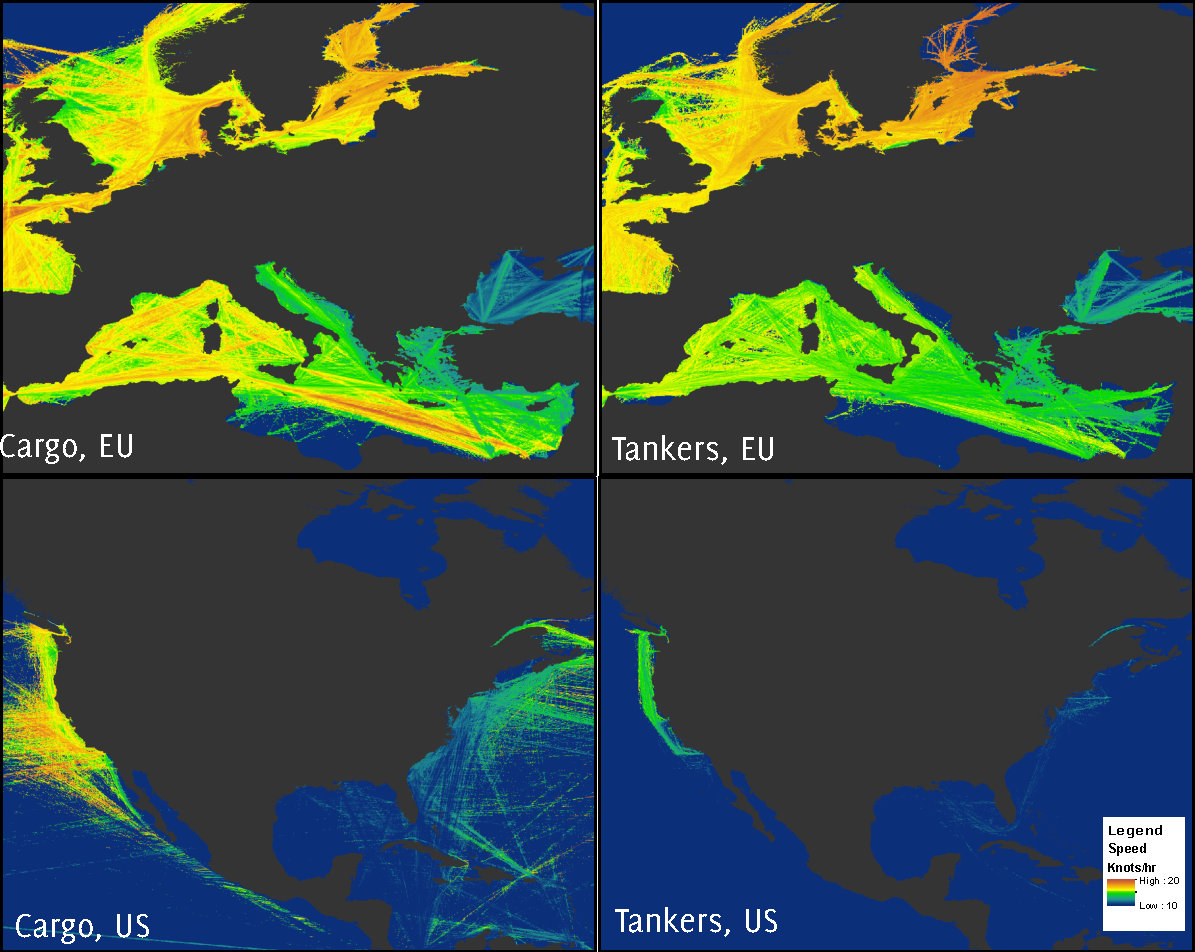
\includegraphics[width=160mm]{images/speed_map_labeled.pdf}}
  \caption{Average ship speed examples. Scale shows 10-20 Kts/hr range for all vessels. Of note is the large difference in speeds between the opposite shores of North America.}
  \label{fig:speed-ship-map}
\end{figure}

\subsubsection{Density}

The density maps show the dramatically different movement structure of the major vessel classes: cargo, tankers and passenger ships all exhibit important differences in their movement. 

\begin{figure}[htbp]
  \centerline{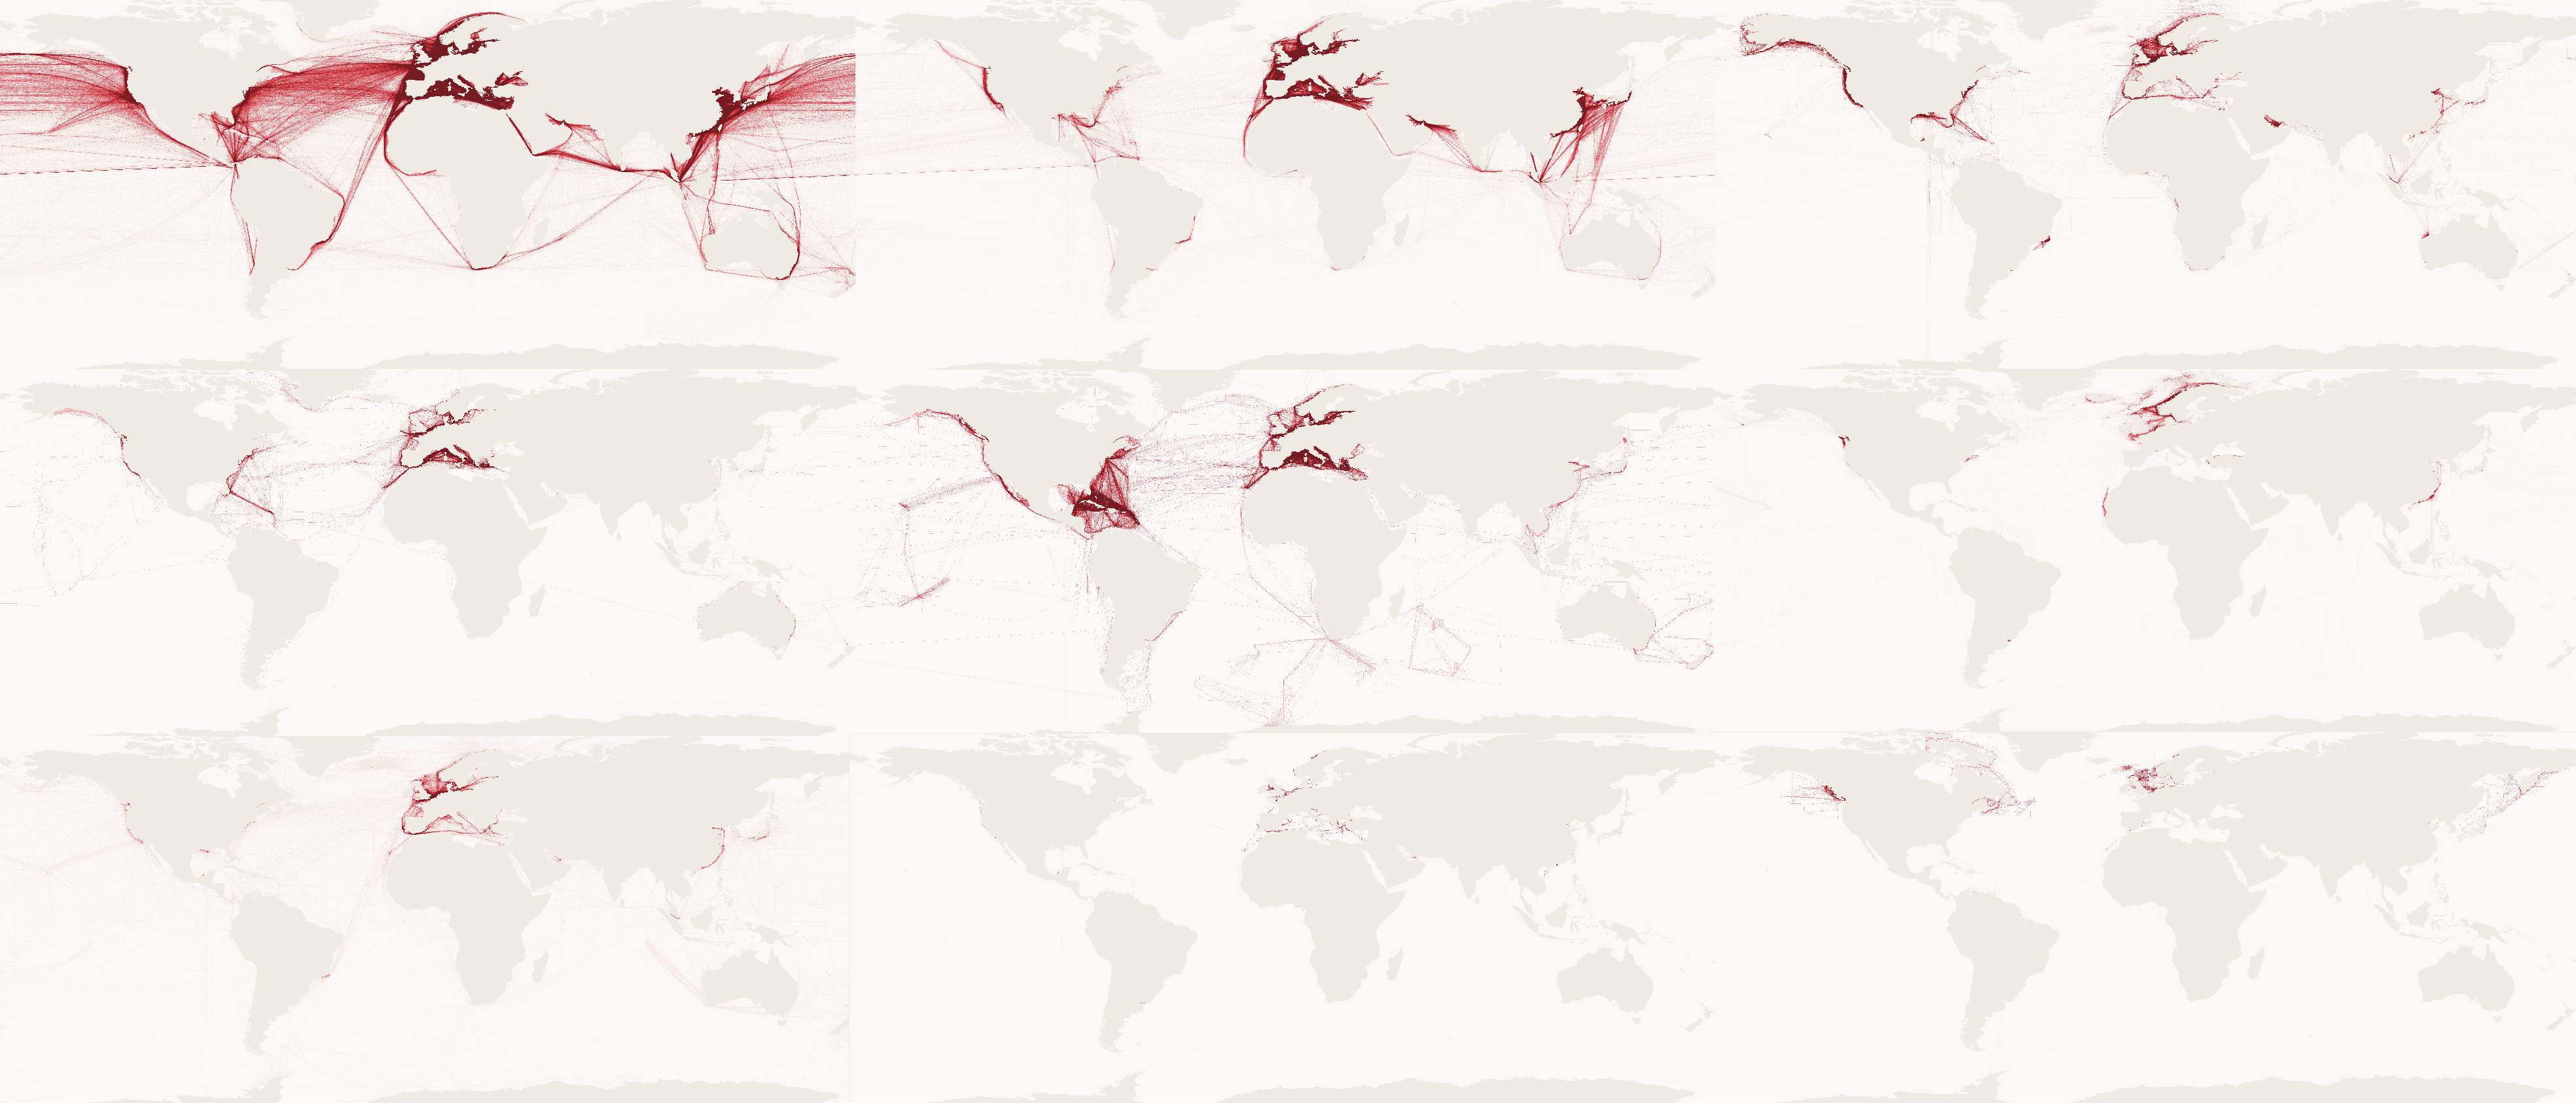
\includegraphics[width=220mm]{figures/9fold-map-black-test_cropped_inverted_thesis.png}}
  \caption{Ship movement densities. first row: cargo, tankers, support. second row:  pleasure, passenger, fishing. third row: other, high-speed, authority.}
  \label{fig:9fold-ship-maps}
\end{figure}


\subsubsection{Spatial Autocorrelation}

Geographic features tend to be clustered, exhibiting spatial autocorrelation. Here, we use Moran's I to compute global autocorrelation statistics for our density rasters:
\begin{equation}
I = \frac{n}{\sum_{i=1}^{n}\sum_{j=1}^{n}w_{ij}}
\frac{\sum_{i=1}^{n}\sum_{j=1}^{n}w_{ij}(x_i-\bar{x})(x_j-\bar{x})}{\sum_{i=1}^{n}(x_i - \bar{x})^2}
\end{equation}

where $n$ is the number of cells, and $w_{ij}$ is the spatial weight.

% XXX: suggestion-- ships by season? just static results here, can do some dynamic stuff later.
